\documentclass[cn,11pt,chinese]{elegantbook}

\title{\,量子场论笔记}
\subtitle{Notes on Quantum Field Theory}

\author{兴趣使然的场论爱好者}
%\bioinfo{录入}{渤海玉兔}
%\institute{Elegant\LaTeX{} Program}
\date{\today}
%\version{3.10}


\extrainfo{The effort to understand the universe is one of the very few things which lifts human life a little above the level of farce and gives it some of the grace of tragedy. --- Steven Weinberg}

%\logo{logo-blue.png}
\cover{Particle.jpeg}

% 本文档命令
%\usepackage[lcgreekalpha]{stix2}
\usepackage{array}
\usepackage{dsfont}
\usepackage{tensor}

\usepackage{pgfplots}
\usepgfplotslibrary{polar}
     \usepgflibrary{shapes.geometric}
     \usetikzlibrary{calc}



\allowdisplaybreaks[4]

 \definecolor{foo}{RGB}{173,34,48}
%+++++++++++++++++++++++数学字体的设置++++++++++++++++++++++++++++++++++++++++%
\newcommand{\me}{\mathrm{e}}  % for math e
\newcommand{\mi}{\mathrm{i}} % for math i
\newcommand{\dif}{\mathrm{d}} %for differential operator d
\newcommand{\cvec}[1]{\!\vec{\,#1}}
\newcommand{\Ptimes}{\,\overset{\otimes }{,}\,}
\DeclareSymbolFont{lettersA}{U}{txmia}{m}{it}
\DeclareMathSymbol{\piup}{\mathord}{lettersA}{25}
 \DeclareMathSymbol{\muup}{\mathord}{lettersA}{22}
 \DeclareMathSymbol{\deltaup}{\mathord}{lettersA}{14}
 \newcommand{\uppi}{\piup}
\newcommand{\ccr}[1]{\makecell{{\color{#1}\rule{1cm}{1cm}}}}


\DeclareFontEncoding{LS1}{}{}
\DeclareFontSubstitution{LS1}{stix}{m}{n}
\DeclareSymbolFont{symbols2}{LS1}{stixfrak}{m}{n}
\DeclareMathSymbol{\typecolon}{\mathbin}{symbols2}{"25}
% 修改目录深度
\setcounter{tocdepth}{2}

\begin{document}

\maketitle
\frontmatter
\mainmatter

\tableofcontents



\renewcommand*\thesection{\arabic{section}}
\setcounter{section}{0}%更改chapter的计数器值
%\numberwithin{equation}{chapter}%公式计数器从属于节计数器
\numberwithin{equation}{section}%公式计数器从属于节计数器
\numberwithin{figure}{chapter}%图计数器从属于节计数器
%\renewcommand*\thefigure{\arabic{section}}
\setcounter{chapter}{0}


\chapter[瞬子]{瞬子\footnote{基于Sidney Coleman, {\textit{The Uses of Instantons}}.}}

\section{简介} \label{instanton:sec1}

考虑四维闵可夫斯基空间中的单个标量场, 其拉格朗日量是
\begin{equation}
    \mathscr{L}=\tfrac{1}{2}\partial_{\mu}\phi \partial^{\mu}\phi
    -\tfrac{1}{2}m^{2}\phi^{2}-g^{2}\phi^{4} \:.
\end{equation}
对于经典物理, $g$是无关参量. 可以定义
\begin{equation}
    \phi'=g\phi\:.
\end{equation}
写成$\phi'$, 
\begin{equation}
    \mathscr{L}=\frac{1}{g^{2}}\Bigl(\tfrac{1}{2}\partial_{\mu}\phi' \partial^{\mu}\phi'
    -\tfrac{1}{2}m^{2}\phi'^{2}-\phi'^{4} \Bigr)\:.
\end{equation}
因此场方程中没有$g$; 如果对任何正的$g$解出了这个理论, 就对其它所有正的$g$解出了这个理论; 所以$g$是无关的. 看到这点的另一个方法是: $g$在经典物理中是{\kaishu{有}}量纲的, 所以可被选为1.

在量子物理中, 由于引入了新常数$\hbar$, $g${\kaishu{是}}相关的, 而重要的物理量是
\begin{equation}
    \mathscr{L}/\hbar = \frac{1}{g^{2}\hbar}\Bigl(\tfrac{1}{2}\partial_{\mu}\phi' \partial^{\mu}\phi'
    -\tfrac{1}{2}m^{2}\phi'^{2}-\phi'^{4} \Bigr) \:.
\end{equation}
我们在这个表达式中看到, 相关(无量纲)参量是$g^{2}\hbar$, 因此半经典近似, 即小$\hbar$近似, 等同于弱耦合近似, 也就是小$g$近似.

我们有一个足以胜任的小耦合近似微扰论吗? 答案是否定的; 有许多有趣的现象在耦合常数很小时发生了但微扰论并不足以解释它们.

看到这点的最简单方法是从场论退回到力学. 考虑在一维势下运动的质量为1的粒子,
\begin{equation}
    L=\tfrac{1}{2}\dot{x}^{2}-V(x;g) \:, 
\end{equation}
其中
\begin{equation}
    V(x;g)=\frac{1}{g^{2}} F(gx) \:,
\end{equation}
而函数$F$的Taylor展开中的领头项是$x^{2}$阶的. 我们来考虑穿越势垒的跃迁现象(见图\ref{instantonfig1}). 
\begin{figure}[h]
    \centering
    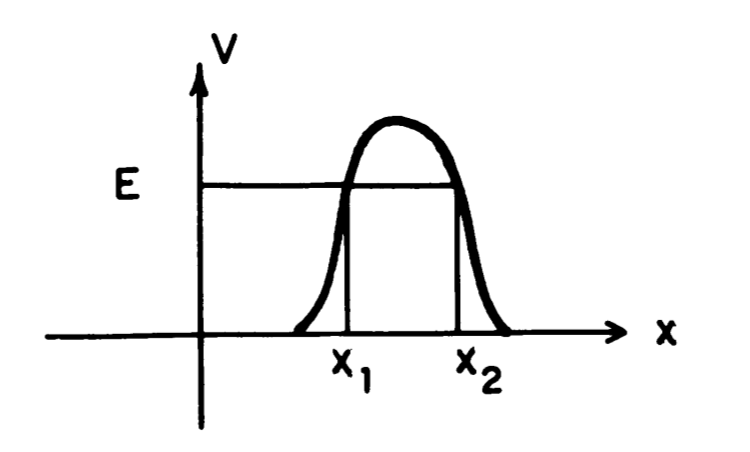
\includegraphics[width=0.6\textwidth]{instantonfig1.jpeg}
    \caption{ \label{instantonfig1}}
  \end{figure}

我们都知道这个跃迁振幅服从WKB公式
\begin{equation}
    \bigl\lvert T(E)\bigr\rvert =\exp\biggl(-\frac{1}{\hbar}\int_{x_{1}}^{x_{2}}\dif x\: \sqrt{2(V-E)}\biggr)[1+O(\hbar)] \:, \label{instanton1.7}
\end{equation}
其中$x_{1}$和$x_{2}$使得这个区域内的$V(x)$大于$E$. 
\begin{tcolorbox}
    一个非常简单的解释: 波函数可以近似写为$\exp(\mi p x/\hbar)$, 而$E=\frac{1}{2}p^{2}+V$, 所以在$E<V$时, $p=\mi\sqrt{2(V-E)}$, 波函数指数衰减.
\end{tcolorbox}
然而, 这个势垒隧穿在微扰论的任何阶都没有看到, 这是因为方程\eqref{instanton1.7}比$\hbar$的任意幂次都衰减的快, 因此也就比$g$的任意幂次都衰减得快.

在量子场论中, 尤其是量子色动力学中, 有类似于量子力学中的隧穿现象的效应, 这也就是所谓的瞬子.

{\heiti{符号说明}}: 时空特征是$({+}{-}{-}{-})$, $x^{0}$是时间坐标, $g_{\mu\nu}$是时空度规, $x^{4}=-\mi x^{0}$是到欧几里得时空的延拓.

\section{粒子力学中的瞬子和回弹} \label{instanton:sec2}

\subsection{欧几里得泛函积分} \label{instanton:sec2.1}

在本节我们继续处理单位质量的无自旋粒子在一维势下运动的理论:
\begin{equation}
    H = \frac{p^2}{2} + V(x) \:. \label{instanton2.1}
\end{equation}
这是一个量子力学问题, 但我们不采用处理这类问题的标准方法, 而是容易推广到量子场论的方法.

我们的基本工具是Feynman历史求和的欧几里得版:
\begin{equation}
    \langle x_{f} \vert \me^{-HT/\hbar} \vert x_{i}\rangle =N \int [\dif x]\, \me^{-S/\hbar} \:. \label{instanton2.2}
\end{equation}
方程\eqref{instanton2.2}左边的$\lvert x_{i}\rangle$和$\lvert x_{f}\rangle$是位置本征态, $H$是哈密顿量, 而$T$是一个正数. 利用能量本征态
\begin{equation}
    H\vert n \rangle = E_{n} \vert n\rangle \label{instanton2.3}
\end{equation}
展开方程\eqref{instanton2.2}左边, 那么就有
\begin{equation}
    \langle x_{f} \vert \me^{-HT/\hbar} \vert x_{i}\rangle 
    = \sum_{n}\me^{-E_{n}T/\hbar}  \langle x_{f} \vert n\rangle \langle n \vert x_{i}\rangle  \:. \label{instanton2.4}
\end{equation}
这个展开在大$T$时的领头项给出了能量最低的本征态的能量和波函数.

在方程\eqref{instanton2.2}右边, $N$是归一化常数, $S$是欧几里得作用量
\begin{equation}
    S=\int_{-T/2}^{T/2} \dif t\:\biggl[\frac{1}{2}\biggl(\frac{\dif x}{\dif t}\biggr)^{2}+V\biggr] \:, \label{instanton2.5}
\end{equation}
而$[\dif x]$代表对所有满足边界条件$x(-T/2)=x_{i}$和$x(T/2)=x_{f}$的函数$x(t)$积分. 更具体一些, 如果$\overline{x}$是满足边界条件的任意函数, 那么满足边界的一般函数可以写成
\begin{equation}
    x(t)=\overline{x}(t)+\sum_{n}c_{n}x_{n}(t) \:, \label{instanton2.6}
\end{equation}
其中$x_{n}$是在边界处为零的实正交函数完备集,
\begin{subequations}\label{instanton2.7}
    \begin{gather}
        \int_{-T/2}^{T/2} \dif t\: x_{n}(t)x_{m}(t) = \delta_{nm} \:, \label{instanton2.7a} \\
        x_{n}(\pm T/2)=0 \:.  \label{instanton2.7b}
    \end{gather}
\end{subequations}
这样, 测度就定义成
\begin{equation}
    [\dif x] = \prod_{n} (2\pi\hbar)^{-1/2} \dif c_{n} \:. \label{instanton2.8}
\end{equation}
(这里的归一化常数$N$依赖于测度的定义, 但是归一化常数会抵消, 所以不需要它的准确定义.)

方程\eqref{instanton2.2}右边可以用半经典(小$\hbar$)极限计算. 在这个情况下, 泛函积分由$S$的稳定点主导. 简单起见, 我们假定只有一个这样的稳定点, 我们将其记为$\overline{x}$, 它满足牛顿方程
\begin{equation}
    \frac{\delta S}{\delta x}\biggr\vert_{x=\overline{x}} = 
    -\frac{\dif^{2}\overline{x}}{\dif t^{2}} + V'(\overline{x}) = 0 \label{instanton2.9}
\end{equation} 
其中加撇号代表对$x$的导数. 更进一步, 我们令$x_{n}$是$S$在$\overline{x}$处的二阶变分导数的本征函数,
\begin{equation}
    -\frac{\dif^{2} x_{n}}{\dif t^{2}} + V''(\overline{x})x_{n} = \lambda_{n}x_{n} \:. \label{instanton2.10} 
\end{equation}
那么, 在小$\hbar$极限下, 这个积分变成高斯积分的乘积, 所以有
\begin{align}
    \langle x_{f} \vert \me^{-HT/\hbar} \vert x_{i}\rangle 
   & = N \me^{-S(\bar{x})/\hbar}\prod_{n}\lambda_{n}^{-1/2}[1+O(\hbar)] \nonumber \\
   &= N \me^{-S(\bar{x})/\hbar}\Bigl[\det\bigl(-\partial_{t}^{2}+V''(\overline{x})\bigr)\Bigr]^{-1/2}[1+O(\hbar)] \:. \label{instanton2.11}
\end{align}
如果有数个稳定点, 一般需要求和.
\begin{tcolorbox}
    这里解释一下方程\eqref{instanton2.10}和\eqref{instanton2.11}, 在$\overline{x}$附近展开$S$, 并设微扰为$\eta$, 那么
    \begin{align*}
        \delta S&= S(\overline{x}+\eta)-S(\overline{x}) 
        = \int \dif t\, \Bigl(\tfrac{1}{2}\bigl(\dot{\overline{x}}+\dot{\eta}\bigr)^{2}+V(\overline{x}+\eta)-\tfrac{1}{2}\dot{\overline{x}}^{2}-V(\overline{x})\Bigr) \\
        &=\int \dif t\,\Bigl(\dot{\overline{x}}\dot{\eta}- V'(\overline{x})\eta+\tfrac{1}{2}\dot{\eta}^{2}+\tfrac{1}{2}V''(\overline{x})\eta^{2}+O(\eta^{2})\Bigr)
        =\frac{1}{2}\int \dif t\, \eta(-\partial_{t}^{2}+V'')\eta
    \end{align*}
在最后一个等号这里使用了牛顿方程\eqref{instanton2.9}, 分部积分并忽略了$\eta$的高阶项. 

用$(-\partial_{t}^{2}+V'')$的本征函数完备集$\{x_{n}\}$展开$\eta=\sum c_{n}x_{n}$, 利用方程\eqref{instanton2.7}就得到了
\begin{equation*}
    \delta S= \frac{1}{2} \lambda_{n}c_{n}^{2}
\end{equation*}
那么
\begin{align*}
    N \int [\dif x]\, \me^{-S/\hbar}&=N \me^{-S(\overline{x})/\hbar} \int [\dif x]\, \me^{-\delta S/\hbar} \\
    &=N \me^{-S(\overline{x})/\hbar} \int \prod_{n} (2\pi\hbar)^{-1/2} \dif c_{n}\:\me^{-\frac{1}{2} \lambda_{n}c_{n}^{2}/\hbar}
    =N \me^{-S(\overline{x})/\hbar}\prod_{n} \lambda_{n}^{-1/2} .
\end{align*}
\end{tcolorbox}

根据方程\eqref{instanton2.9}, 能量是
\begin{equation}
    E=\frac{1}{2}\biggl(\frac{\dif\overline{x}}{\dif t}\biggr)^{2} - V(\overline{x})
\end{equation}
这可以用来决定方程\eqref{instanton2.9}的解的定性性质.

\begin{figure}[h]
    \centering
    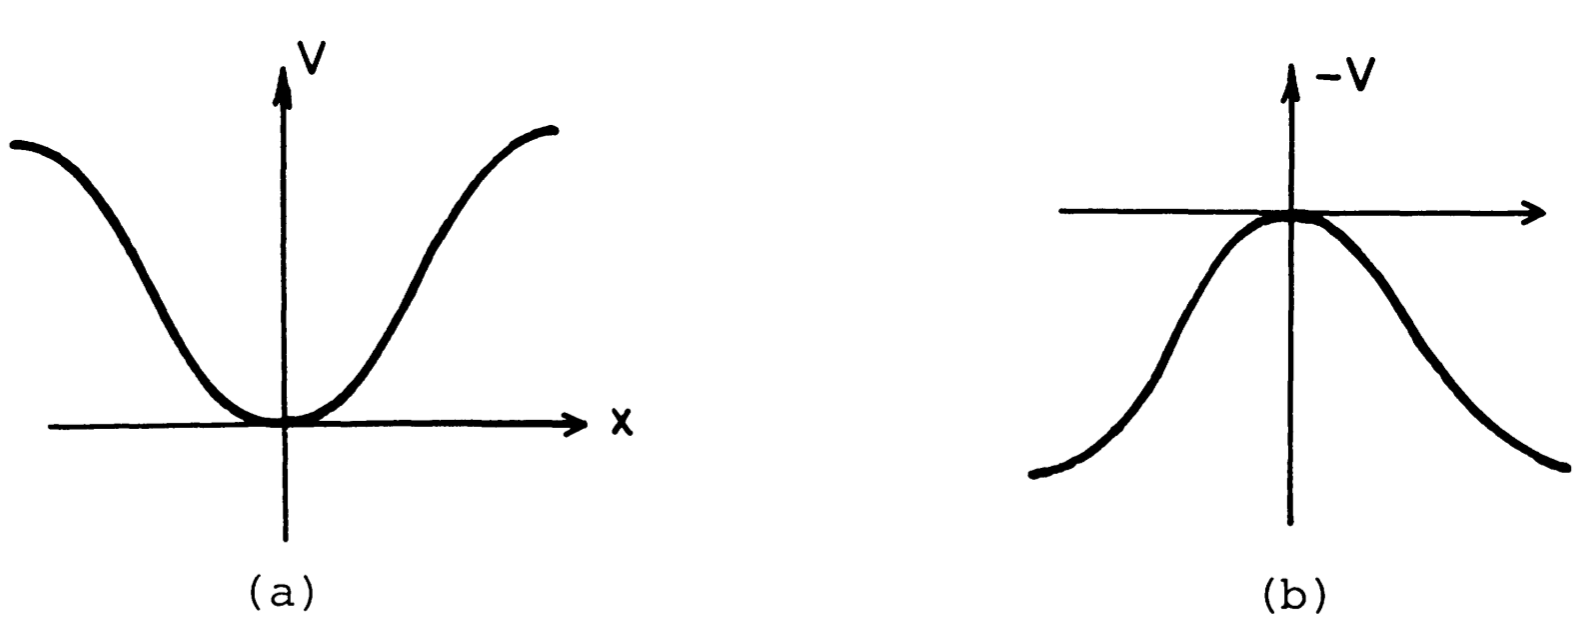
\includegraphics[width=0.8\textwidth]{instantonfig2.jpeg}
    \caption{ \label{instantonfig2}}
  \end{figure}
作为一个简单例子, 考虑图\ref{instantonfig2}(a)中的势能. 选择$x_{i}=x_{f}=0$. 方程\eqref{instanton2.9}满足边界条件的解显然是
\begin{equation}
    \overline{x}=0 . \label{instanton2.13}
\end{equation}
对于这个解, $S(\overline{x})=0$. 那么, 从方程\eqref{instanton2.11}
\begin{equation}
    \langle 0 \vert \me^{-HT/\hbar} \vert 0\rangle = 
    N[\det(-\partial_{t}^{2}+\omega^{2})]^{-1/2}[1+O(h)] \:, \label{instanton2.14}
\end{equation}
其中
\begin{equation}
    \omega^{2}=V''(0) \:. \label{instanton2.15}
\end{equation}

可以证明, 对于很大的$T$,
\begin{equation}
    N[\det(-\partial_{t}^{2}+\omega^{2})]^{-1/2} \simeq \biggl(\frac{\omega}{\pi\hbar}\biggr)^{1/2}\me^{-\omega T/2}.  \label{instanton2.16}
\end{equation}
根据方程\eqref{instanton2.4}, 基态能量是
\begin{equation}
    E_{0}=\frac{1}{2}\omega\hbar[1+O(\hbar)] \:. \label{instanton2.17}
\end{equation}
同理, 基态粒子处在原点的几率是
\begin{equation}
     \bigl\lvert \langle x{=}0 \vert n{=}0 \rangle \bigr\rvert^{2} =
     (\omega/\pi\hbar)^{1/2}[1+O(\hbar)] .
\end{equation}

这些当然是正确的半经典结果. 在小$\hbar$极限下, 粒子处在位于原点的谐振子基态中, 能量就是谐振子的基态能量.

\begin{tcolorbox}[breakable]
    推导方程\eqref{instanton2.16}的两种方法:

    (1)蛮干法(Poor man's way): 求解如下微分方程
\[
 (-\partial_{t}^{2}+\omega^{2})f= \lambda_{n}f
\]
由于$f$要满足边界条件$f(\pm T/2)=0$, 所以$\lambda_{n}>\omega^{2}$, 并要满足
\[
 \sqrt{\lambda_{n}-\omega^{2}} = \frac{n\pi}{T}    
\]
那么根据方程\eqref{instanton2.11}, 
\begin{align*}
    [\det(-\partial_{t}^{2}+\omega^{2})]^{-1/2}
    =\prod_{n}\biggl(\frac{n^{2}\pi^{2}}{T^{2}}+\omega^{2}\biggr)^{-1/2}
\end{align*}
上式需要重整化, 除以一个不依赖于$\omega$的无限大常数$[\det(-\partial_{t}^{2})]^{-1/2}$, 得到
\begin{align*}
    [\det(-\partial_{t}^{2}+\omega^{2})]^{-1/2}&=\prod_{n}\Biggl(
        1+ \biggl(\frac{\omega T}{n\pi}\biggr)^{2}\Biggr)^{-1/2} \\
        &= \biggl(\frac{\sinh(\omega T)}{\omega T}\biggr)^{-1/2}
\end{align*}
在$T$很大时, $\sinh(\omega T)\simeq \me^{\omega T}$. 常数$N$可以通过考虑自由粒子来决定, 这里不再赘述.

(2) Coleman的方法, 根据定义
\[
\det(-\partial_{t}^{2}+W)=\prod_{n}\lambda_{n}    
\]
其中$\lambda_{n}$是算符$(-\partial_{t}^{2}+W)$的本征值, 那么$(-\partial_{t}^{2}+W-\lambda)$的本征值是$\lambda_{n}-\lambda$. 这样就有
\[
\frac{\det(-\partial_{t}^{2}+W^{(1)}-\lambda)}{\det(-\partial_{t}^{2}+W^{(2)}-\lambda)}  = \frac{\psi_{\lambda}^{(1)}(T/2)}{\psi_{\lambda}^{(2)}(T/2)}  .
\]
这里$\psi$满足
$(-\partial_{t}^{2}+W^{(i)})\psi_{\lambda}^{(i)}=\lambda \psi_{\lambda}^{(i)}$以及边界条件$\psi_{\lambda}(-T/2)=0$和$\dot{\psi}_{\lambda}(-T/2)=1$. 显然$\psi_{\lambda}^{(i)}$只有$\lambda=\lambda_{n}$时满足边界条件$\psi_{\lambda}^{(i)}(\pm T/2)=0$. 将上式左右两边视为$\lambda$的函数, 那么左右两边就有相同的零点和极点, 所以相等.

由此可得
\[
    \frac{\det(-\partial_{t}^{2}+W)}{\psi_{0}(T/2)} =\text{常数} = \pi\hbar N^{2} 
\]
其中$N$是一个常数. (这也是Coleman对$N$的定义.) 对于$W=\omega^{2}$, 可以解出
\[
\psi_{0}=\omega^{-1} \sinh \omega(t+T/2)\:,   
\]
进而也就得到了方程\eqref{instanton2.16}

\end{tcolorbox}


\subsection{双井与瞬子} \label{instanton:sec2.2}

我们现在转向不那么平庸的问题, 图\ref{instantonfig3}(a)所示的双井. 假定势是偶函数, $V(x)=V(-x)$, 它的最小值点记为$\pm a$. 选择一个常数, 使得$V$的最小值是0, 并将$V''(\pm a)$记为$\omega^{2}$.
\begin{figure}[h]
    \centering
    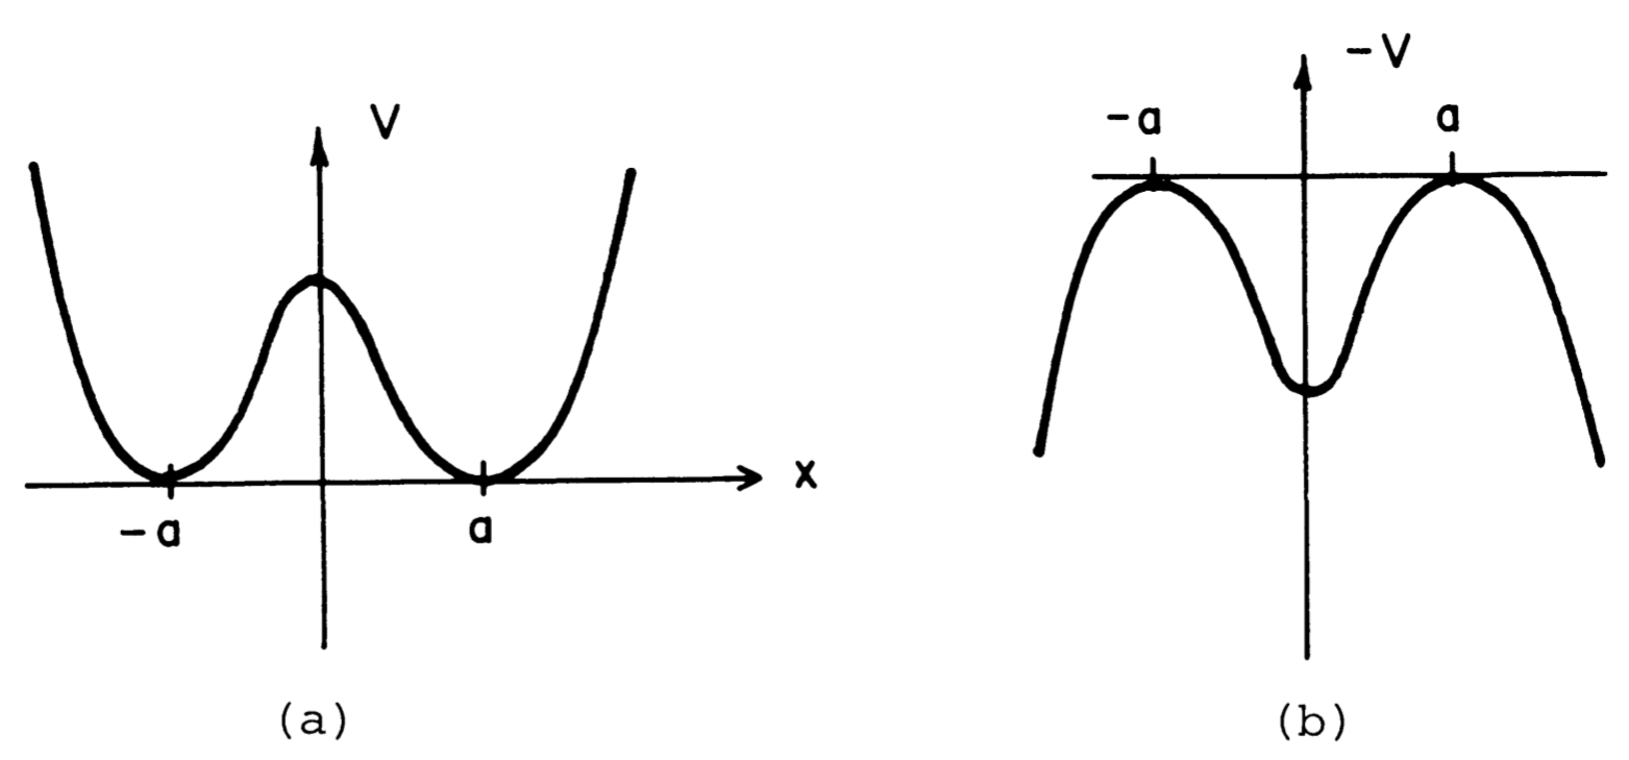
\includegraphics[width=0.8\textwidth]{instantonfig3.pdf}
    \caption{ \label{instantonfig3}}
\end{figure}

我们将尝试计算
\begin{subequations}
    \begin{align}
        \langle {-}a \vert \me^{-HT} \vert {-}a \rangle &= \langle a \vert \me^{-HT} \vert a \rangle \:, \label{instanton2.19a}\\ 
        \langle a \vert \me^{-HT} \vert {-}a \rangle &= \langle {-}a \vert \me^{-HT} \vert a \rangle \:,\label{instanton2.19b}
    \end{align}
\end{subequations}
方法是通过半经典极限方程\eqref{instanton2.11}来近似泛函积分. 和前面一样, 先求解与边界条件相容的经典欧几里得运动方程, \eqref{instanton2.9}. 

当然, 两个这样的解是粒子待在两个井底(或者说图\ref{instantonfig3}(b)的两个山顶). 然而还有另一种有趣的解, 在$-T/2$时待在其中一个山顶, 然后在$T/2$时跑到另一个山顶.
由于我们最后会把$T$取为无穷大, 我们将专注于这个极限下的解形式, 即粒子在无穷远的过去从一个山顶离开, 然后在无穷远的未来达到另一个山顶. 在这个情况下, 运动方程的解的能量为零; 
所以
\begin{equation}
    \dif x/\dif t =\sqrt{2V}. \label{instanton2.20}
\end{equation}
等效地有
\begin{equation}
    t= t_{1}+\int_{0}^{x}\dif x' \: (2V)^{-1/2} \:, \label{instanton2.21}
\end{equation}
其中$t_{1}$是积分常数, $x(t_{1})$为零.

\begin{figure}[h]
    \centering
    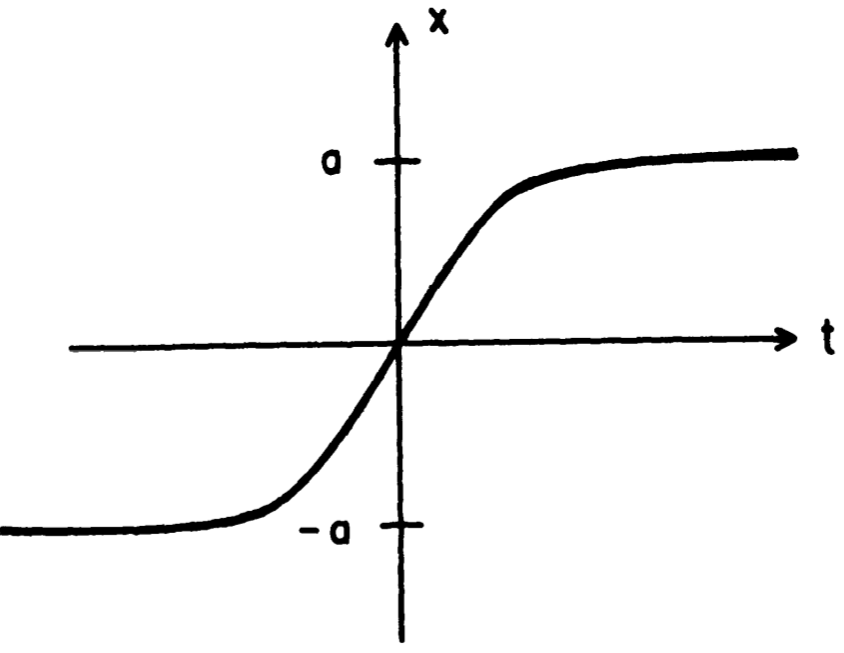
\includegraphics[width=0.5\textwidth]{instantonfig4.jpeg}
    \caption{ \label{instantonfig4}}
  \end{figure}

解的图示参看图\ref{instantonfig4}; 它被称为``中心在$t_{1}$的瞬子''. 瞬子这一词汇是't Hooft发明的. 灵感来源于它们的数学结构十分类似于所谓的孤子(solitons)或鼓包(lump), 
经典场论的类粒子解: 因此称为``-子''. 然而, 不像鼓包, 它们在时间(尽管是欧几里得时间)中是局域的: 因此是``瞬-''. 由于相同的原因, Polyakov称其为``赝粒子(pseudoparticle)'', 也见于文献.

当然, 我们可以也可以构建从$a$到${-}a$的解, 将方程\eqref{instanton2.21}中的$t$换为$-t$即可; 它们被称为``反瞬子''.

这些解有两个很重要的性质:
\begin{enumerate}
    \item 从方程\eqref{instanton2.20}可以导出瞬子(或反瞬子)作用量的一个简单表达式
    \begin{equation}
        S_{0}=\int \dif t\:\bigl[\tfrac{1}{2}\dot{x}^{2}+V\bigr] =\int \dif t \: \dot{x}^{2} = \int_{-a}^{a}\dif x\:\sqrt{2V} \:. \label{instanton2.22}
    \end{equation}
    注意这与势垒隧穿公式\eqref{instanton1.7}中出现的积分相同. 我们会在后面看到这不是个巧合.
    \item 对于大$t$, $x$趋于$a$, 方程\eqref{instanton2.20}可以近似为
    \begin{equation}
        \dot{x} = \omega(a-x) \:. \label{instanton2.23}
    \end{equation}
    因此, 对于大$t$,
    \begin{equation}
        (a-x) \propto \me^{-\omega t} \:. \label{instanton2.24}
    \end{equation}
    因此瞬子是一个非常定域的物体, 它的尺寸大约是$1/\omega$阶的.
\end{enumerate}

这是十分重要的, 因为这意味着: 当$T$很大时, 瞬子和反瞬子不仅是运动方程的近似解; 相距甚远的瞬子和反瞬子串联而成的场构型也是近似解. 

泛函积分将通过对所有这样的构型求和计算, 其中每个构型有$n$个物体(瞬子或反瞬子), 中心处在$t_{1},\ldots,t_{n}$, 其中
\begin{equation}
    T/2>t_{1}>\cdots>t_{n}>-T/2\:. \label{instanton2.25}
\end{equation}

图\ref{instantonfig5}展示了这样一个构型. $T$相比于瞬子尺寸要大很多; 因此图\ref{instantonfig4}的光滑曲线在图5的尺度上就变成了尖锐的跃变. 

\begin{figure}[h]
    \centering
    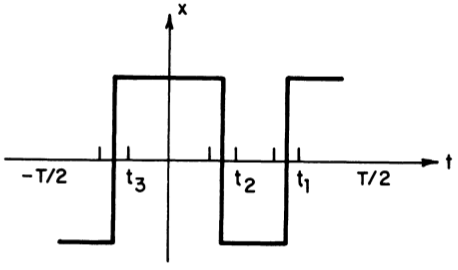
\includegraphics[width=0.6\textwidth]{instantonfig5.jpeg}
    \caption{ \label{instantonfig5}}
  \end{figure}

现在是计算:
\begin{enumerate}
    \item 对于$n$个相距甚远的物体, $S$就是$n S_{0}$. 要考虑到作用量在指数上.
    \item 泛函行列式的计算需要一些技巧. 我们把时间演化算符$\me^{-HT}$视为图\ref{instantonfig5}中时间轴上垂直线所标出的点之间的演化算符的乘积. 
    要不是存在含有瞬子和反瞬子的小区间, $V''$在整个时间上等于$\omega^{2}$, 因此我们所获得的结果与\ref{instanton:sec2.1}节中的单井势的结果相同, 
    \begin{equation}
        \biggl(\frac{\omega}{\pi\hbar}\biggr)^{1/2} \me^{-\omega T/2} \:. \label{instanton2.26}
    \end{equation}
    含有瞬子和反瞬子的小区间修正了这个公式. 因此我们得到
    \begin{equation}
        \biggl(\frac{\omega}{\pi\hbar}\biggr)^{1/2} \me^{-\omega T/2}K^{n} \:. \label{instanton2.27}
    \end{equation}
    其中$K$可以通过计算只有一个瞬子的情况得到.
    \item 我们必须要对瞬子中心所处的位置的积分:
    \begin{equation}
        \int_{-T/2}^{T/2} \dif t_{1}\int_{-T/2}^{t_{1}} \dif t_{2} \cdots \int_{-T/2}^{t_{n-1}} \dif t_{n} 
        =T^{n}/n! \:. \label{instaton2.28}
    \end{equation}
    \item 我们无法自由地分配瞬子和反瞬子. 例如, 如果我们从${-}a$出发, 那么第一个遇到的物体必然是瞬子, 下一个必然是反瞬子, 以此类推. 
    更进一步, 如果我们最后返回${-}a$, $n$必须是偶数. 同样, 如果我们最后停到了$a$, $n$必须是奇数. 
\end{enumerate}

因此,
\begin{equation}
    \langle{-}a\vert \me^{-HT/\hbar} \vert {-a}\rangle 
    =\biggl(\frac{\omega}{\pi\hbar}\biggr)^{1/2} \me^{-\omega T/2} 
    \sum_{\text{even }n} \frac{\bigl(K\me^{-S_{0}/\hbar}T\bigr)^{n}}{n!}[1+O(\hbar)] \:, \label{instanton2.29}
\end{equation}
而$\langle a\vert \me^{-HT/\hbar} \vert {-a}\rangle $由只对奇数$n$求和的相同表达式给出. 这些求和是平庸的:
\begin{equation}
    \langle \pm a\vert \me^{-HT/\hbar} \vert {-a}\rangle 
    =\frac{1}{2}\biggl(\frac{\omega}{\pi\hbar}\biggr)^{1/2} \me^{-\omega T/2}
    \Bigl[\exp\bigl(K\me^{-S_{0}/\hbar}T\bigr)\pm \exp\bigl(-K\me^{-S_{0}/\hbar}T\bigr)\Bigr] 
    \:, \label{instanton2.30}
\end{equation}
(从现在起将省略因子$[1+O(\hbar)]$.)

与方程\eqref{instanton2.4}比较, 我们现在有两种能量最底态, 其能量是
\begin{equation}
    E_{\pm} = \tfrac{1}{2}\hbar\omega \pm \hbar K \me^{-S_{0}/\hbar} \:. \label{instanton2.31}
\end{equation}
如果我们把这些本征态记为$\lvert + \rangle$和$\lvert - \rangle$, 我们看到
\begin{equation}
    \bigl \lvert \langle + \vert {\pm} a \rangle \bigr \rvert^{2} = \bigl \lvert \langle - \vert {\pm} a \rangle \bigr \rvert^{2} 
    =\langle a\vert -\rangle \langle - \vert {-}a\rangle =-\langle a\vert +\rangle \langle + \vert {-}a\rangle 
    =\frac{1}{2} \biggl(\frac{\omega}{\pi\hbar}\biggr)^{1/2} \:. \label{instanton2.32}
\end{equation}
当然, 它们是预期的结果: 能量本征态是中心在两个井底的谐振子态在空间上为偶或为奇的组合; 两个能量本征态的简并只被势垒隧穿破坏了(因此能量差正比于势垒隧穿因子$\me^{-S_{0}/\hbar}$), 而能量较低的态, 即我们记为$\lvert -\rangle$的那个, 在空间上为偶的组合. \\
\begin{remark}
设$\vert + \rangle= (m_{+}\lvert 0_{+}\rangle+n_{+}\lvert 0_{-}\rangle)/\sqrt{2}$和$\vert - \rangle= (m_{-}\lvert 0_{+}\rangle+n_{-}\lvert 0_{-}\rangle)/\sqrt{2}$, 其中$\lvert 0_{\pm}\rangle$是中心分别处在$\pm a$的谐振子态. 方程\eqref{instanton2.32}给出$m_{+}=-n_{+}$和$m_{-}=n_{-}$, 以及它们的范数为1.
\end{remark}

下个任务是计算$K$. 在计算之前, 我们先对所做的事情做一些评论:
\begin{enumerate}
    \item 实际上我们没有权利在方程\eqref{instanton2.31}中保留第二项. 不仅是因为它指数式小于第一项, 它也指数式得小于对第一项的未知$O(\hbar^{2})$修正. 然而这是对能量差$E_{+}-E_{-}$的领头阶修正; 一个更加严格的做法是仅在能量差的表达式中保留这一项, 而在单个能量的表达式中略去它.
    \item 我们的近似基于瞬子和反瞬子相距甚远的假定. 作为一个自洽性检验, 我们应该验证最后结果的主要部分来自于这样的构型. 
    
    这个检验很容易做. 对于固定的$x$, 指数系数$\sum x^{n}/n!$中的项随着$n$的增长而增长直到$n$到达$x$的量级, 在这之后, 开始快速衰减. 对方程\eqref{instanton2.29}中的求和应用这个性质, 我们看到重要的项是那些
    \begin{equation}
        n \lesssim KT \me^{-S_{0}/\hbar} \label{instanton2.33}
    \end{equation}
    的项. 这就是说, 对于小$\hbar$, 求和中重要的项是那些瞬子和反瞬子密度$n/T$是指数量级小数的项, 因此平均间隔非常大. 注意到这个平均间隔$K\me^{-S_{0}\hbar}$实际上独立于$T$; 我们的近似实际上是小$\hbar$近似; 只要$T$足够大, 这个条件就独立于$T$而成立.

    瞬子相距甚远这个近似被称为稀薄气体近似.
    \item 最后进一步解释下$S$的近似稳相点这个概念. 我们先来看单变量积分,
    \begin{equation}
        I=\int_{0}^{T} \dif t\: \me^{-S(t)/\hbar} \:, \label{instanton2.34}
    \end{equation}
    其中$S$是$t$的单调递减函数, 它的渐进值是$S(\infty)$. 因此这个被积函数在积分区域中没有稳相点. 然而对于小$\hbar$和大$T$, 很容易找到这个积分的如下近似形式
    \begin{equation}
        I\approx T \me^{-S(\infty)/\hbar} \:. \label{instanton2.35}
    \end{equation}
    大概地讲, 这个积分被无穷远处的稳相点所主导. 将这个现象推广到多维积分是直接的: 我们假定被积函数的图像有某种波谷; 沿着谷底的线会随着我们趋于无穷远而变平. 换言之, 在高维空间中有一条线, 使得被积函数在垂直于线的方向上在该线所处的位置达到最小值, 并在沿着这条线趋于无穷远时达到某个近似值. 当然这个线本身可以推广至超平面. ``近似稳相点''实际上就是这样的情况; 瞬子和反瞬子的所在就是沿着谷底的变量; $S$仅在它们趋于无穷远处变得稳定(并等于$nS_{0}$).
\end{enumerate}
\vspace{0.5cm}
现在我们来计算$K$.

我们现在必须要研究本征方程\eqref{instanton2.10}, 其中$\overline{x}$是单瞬子. 由于时间平移不变性, 这个方程必然有一个本征值为零的本征函数,
\begin{equation}
    x_{1} = S_{0}^{-1/2} \dif \overline{x}/\dif t \:. \label{instanton2.36}
\end{equation}
(归一化因子来自于方程\eqref{instanton2.22}.)
\begin{tcolorbox}
    我们稍微解释一下函数\eqref{instanton2.36}的来源. 这里的时间平移性是指: 当时间$T$是无穷时, 无论单瞬子$\overline{x}$的中心在哪, 作用量$S(\bar{x})$都是相同的. 设中心在$t_{1}$的单瞬子为$\bar{x}(t-t_{1})$, 那么对于两个相距很近的单瞬子, 我们就有
    \begin{equation*}
        0=\delta S= S[\overline{x}(t-t_{1}-\Delta t_{1})]-S[\overline{x}(t-t_{1})]=\frac{1}{2}\int \dif t\, \eta(-\partial_{t}^{2}+V'')\eta
    \end{equation*} 
    其中$\eta=\overline{x}(t-t_{1}-\Delta t_{1})-\overline{x}(t-t_{1})=-\Delta t_{1} \, \dot{\overline{x}}(t-t_{1})$. 由于算符$(-\partial_{t}^{2}+V'')$没有非负本征值, 所以这个$\eta$肯定是这个算符本征值为零的本征函数. 归一化因子是要求
    \begin{equation*}
        \int \dif t\: x_{1}^{2} =1 
    \end{equation*}
    得到的, 其中用到了方程\eqref{instanton2.22}.
\end{tcolorbox}
如果我们要想对方程\eqref{instanton2.6}中的相应展开系数$c_{1}$积分, 我们会遇到无穷大, 但这个积分实际上已经在对瞬子中心的积分\eqref{instaton2.28}中做过了. 
原因是, 瞬子$\overline{x}(t)$的中心移动所产生的微扰是:
\begin{equation}
    \eta =\dot{\overline{x}} \Delta t_{1} \:. \label{instanton2.37}
\end{equation}
而这造成了本征函数展开系数的扰动
\begin{equation}
    \eta =x_{1}\Delta c_{1} \:. \label{instanton2.38}
\end{equation}
因此,
\begin{equation}
    (2\pi\hbar)^{-1/2} \dif c_{1} = (S_{0}/2\pi\hbar)^{1/2} \dif t_{1} \:.
\end{equation}

因此, 在计算泛函行列式时, 我们应该排除零本征值, 但我们应该该$K$引入因子$(S_{0}/2\pi\hbar)^{1/2}$. 因此, 单瞬子对这个跃迁元的贡献是
\begin{equation}
    \langle a \vert \me^{-HT} \vert {-}a\rangle _{\text{one inst.}} =N T  (S_{0}/2\pi\hbar)^{1/2} \me^{-S_{0}/\hbar}
    \bigl(\det\nolimits'[-\partial_{t}^{2}+V''(\overline{x})]\bigr)^{-1/2} \:, \label{instanton2.40}
\end{equation}
其中$\det'$是指在计算行列式时已经排除了零本征值. 与\eqref{instanton2.29}相比较, 我们得到
\begin{equation}
    K= (S_{0}/2\pi\hbar)^{1/2} \Biggl\lvert \frac{\det(-\partial_{t}^{2}+\omega^{2})}{\det'\bigl(-\partial_{t}^{2}+V''(\overline{x})\bigr)} \Biggr\rvert^{1/2} \:.
\end{equation}

一些注解:
\begin{enumerate}
    \item 为了真的把所有元素缝合在一起, 我们应该证明我们所得到的能级分裂公式与通过传统波动力学方法得到的相同. 这个会在附录中解释.
    \item 我们现在来论述算符$-\partial_{t}^{2}+V''(\overline{x})$的本征值都是非负的. 这个算符是Schr\"{o}dinger方程中的算符, 本征值越大的本征函数拥有更多的节点(零点), 或者更多的波峰波谷(这样本征函数的频率也就越高). 瞬子是单调增函数, 它的导数没有节点, 再加上这个导数是这个算符本征值为零的本征函数. 证毕.
    \item $K$正比于$\hbar^{-1/2}$. 这个因子来自于时间平移不变性产生的零模. 稍后我们会分析拥有更大对称群的理论, 对于这些理论, 瞬子有多个这样的零模. 显然, 每个零模都会给一个$\hbar^{-1/2}$因子. 这种对$\hbar$的幂次计数的规则将起到重要作用, 正如第\ref{instanton:sec1}节所解释的那样, 对$\hbar$的幂次计算等同于对耦合常数的幂次计数.
\end{enumerate}

\subsection{周期势}

我们来考虑如图\ref{instantonfig6}(a)所示的周期势. (方便起见, $V$的最小值点被取成了整数.) 如果忽略势垒隧穿, 能量本征态就是无限多个简并态, 每个都集中在某个井底. 
势垒隧穿将单个本征值变成了连续的本征值带; 真正的能量本征态势单位平移的本征态, Bloch波. 我们现在看一下如何用瞬子方法推导这个旧结果.
\begin{figure}[h]
    \centering
    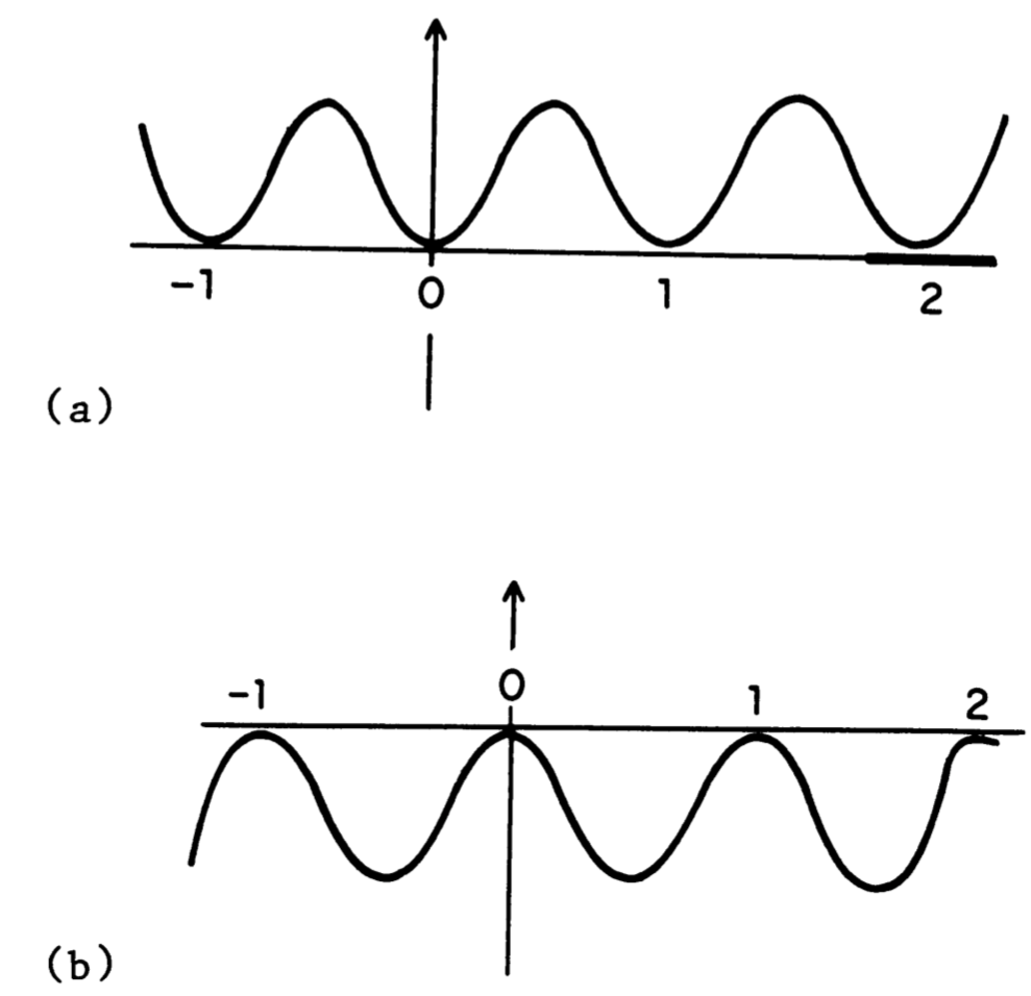
\includegraphics[width=0.5\textwidth]{instantonfig6.pdf}
    \caption{ \label{instantonfig6}}
  \end{figure}

我们从图\ref{instantonfig6}(b)中可以看到, 这里的瞬子和前面的很像. 唯一新的地方是瞬子现在可以从任何初始位置$x=j$出发, 然后去往下一个$x=j+1$. 反瞬子则是从$x=j$到$x=j-1$. 
其余的和之前相同.

因此, 当做稀薄气体求和时, 我们可以在实轴上分布瞬子和反瞬子, 不再有瞬子和反瞬子交替分布这样的约束. 当然, 当我们沿着线行进时, 
每个瞬子或反瞬子都必须从它的前任者的终点出发. 更进一步, 瞬子的总数减去反瞬子的总数必须等于初始位置本征态和终末位置本征态的$x$的变化.

因此我们得到
\begin{equation}
    \langle j_{+} \vert \me^{-HT/\hbar} \vert j_{-} \rangle = \biggl( \frac{\omega}{\pi\hbar}\biggr)^{1/2} \me^{-\omega T/2}
    \sum_{n=0}^{\infty}\sum_{\overline{n}=0}^{\infty} \frac{1}{n!\overline{n}!} \Bigl( K\me^{-S_{0}/\hbar}T\Bigr)^{n+\overline{n}}
    \delta_{n-\overline{n}\,,\,j_{+}-j_{-}} \label{instanton2.42}
\end{equation}
其中$n$是瞬子总数而$\overline{n}$是反瞬子总数. 如果我们使用恒等式
\begin{equation}
    \delta_{a,b}= \int_{0}^{2\pi} \frac{\dif \theta}{2\pi} \:\me^{\mi\theta(a-b)} \:, \label{instanton2.43}
\end{equation}
求和就变成了两个独立的指数级数, 我们发现
\begin{equation}
    \langle j_{+} \vert \me^{-HT/\hbar} \vert j_{-} \rangle = \biggl( \frac{\omega}{\pi\hbar}\biggr)^{1/2} \me^{-\omega T/2}
    \int_{0}^{2\pi}  \frac{\dif \theta}{2\pi} \:\me^{\mi\theta(a-b)}\exp\Bigl[2KT\cos\theta \me^{-S_{0}/\hbar}\Bigr] \:. \label{instanton2.44}
\end{equation}

因此我们得到了用角度$\theta$标记的连续能量本征态. 能量本征值是
\begin{equation}
    E(\theta) = \tfrac{1}{2}h\omega +2 hK \cos\theta \me^{-S_{0}/\hbar} \:. \label{instanton2.45}
\end{equation}
以及
\begin{equation}
    \langle \theta \vert j\rangle =\biggl( \frac{\omega}{4\pi^{3}\hbar}\biggr)^{1/4}  \me^{\mi j\theta} \:. \label{instanton2.46}
\end{equation}
这正是正确结果.

\subsection{非稳态与回弹}

\subsubsection*{伽利略戏仿\footnote{这里仿照了伽利略著作《关于托勒密和哥白尼两大世界体系的对话》的对话体形式, 本节中出现的沙格列陀(Sagredo)和萨尔维阿蒂(Salviati)正是此书中参与对话的两个主要人物, 名字取自伽利略的好友.}} 

\begin{figure}[h]
    \centering
    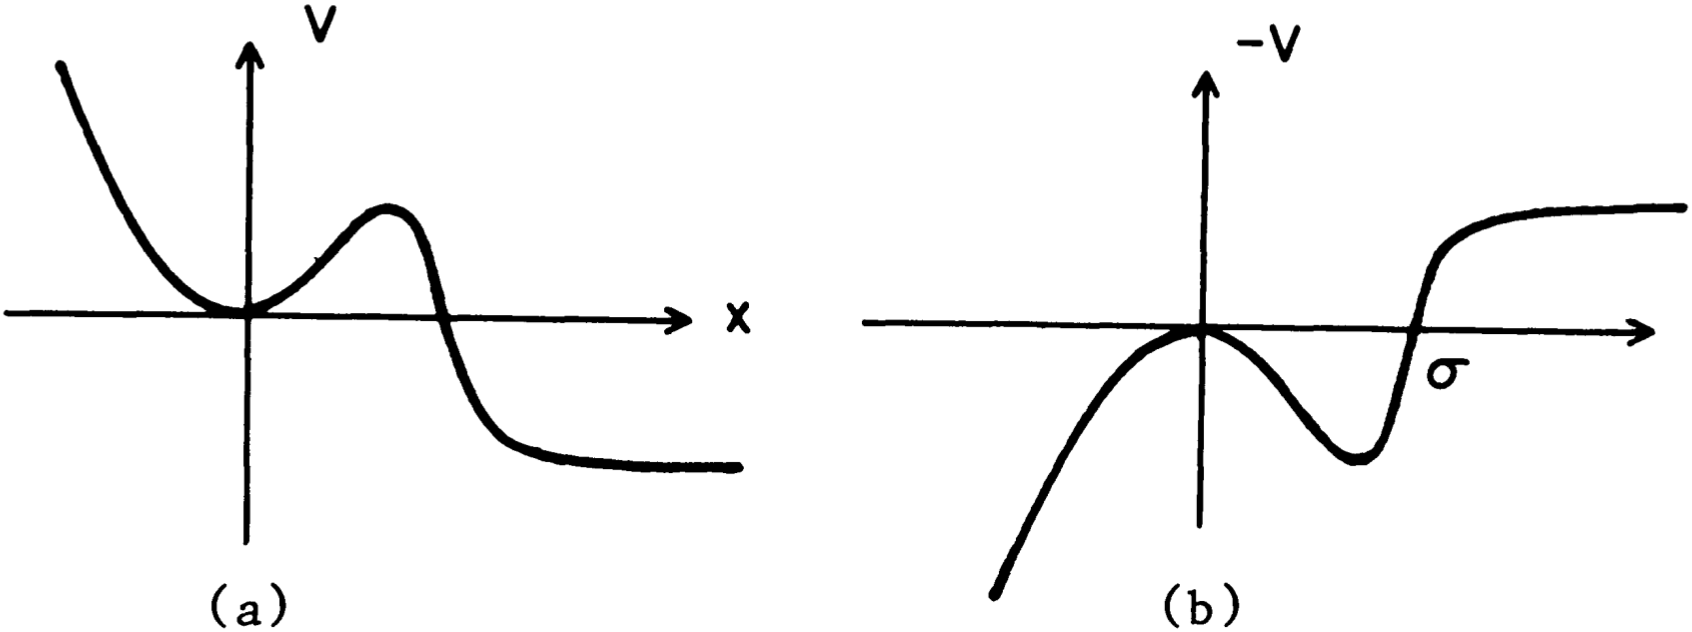
\includegraphics[width=0.7\textwidth]{instantonfig7.png}
    \caption{ \label{instantonfig7}}
  \end{figure}

\noindent {\kaishu{沙格列陀}}: 我想通过用瞬子方法研究图\ref{instantonfig7}(a)中的势以检查我对它们的理解. 如果我忽略势垒隧穿, 在半经典极限下, 这个势有一个处在井底的能量本征态. 我想计算势垒隧穿对这个态的能量的修正. 如果我把这个势上下颠倒(图\ref{instantonfig7}(b)), 我观察到经典运动方程有这样一个解: 粒子从$x=0$处的山顶出发,然后在经典转折点$\sigma$处反弹, 最后回到山顶(图\ref{instantonfig8}). 我们称这种运动为``回弹''(the bounce). 就像在研究双井势时对瞬子和反瞬子求和, 我将通过对相距甚远的回弹构型求和来计算$x=0$和$x=0$之间的跃迁矩阵元. 诚然, 除了对回弹的数目是奇是偶没有限制, 这个求和与双井势的情况相同(这里如何定义$S_{0}$、$\omega^{2}$等是显然的). 因此这里的指数级数是完整的, 而不是只有奇数项或偶数项, 这样就有
\begin{equation}
    \langle 0 \vert \me^{-HT/\hbar} \vert 0 \rangle =\biggl(\frac{\omega}{\pi\hbar}\biggr)^{1/2} \me^{-\omega T/2}
    \exp\bigl[KT \me^{-S_{0}/\hbar}\bigr] \:, \label{instanton2.47}
\end{equation}
而能量本征态是
\begin{equation}
    E_{0}=\tfrac{1}{2}\hbar\omega+\hbar K\me^{-S_{0}/\hbar} \:. \label{instanton2.48}
\end{equation}

\begin{figure}[h]
    \centering
    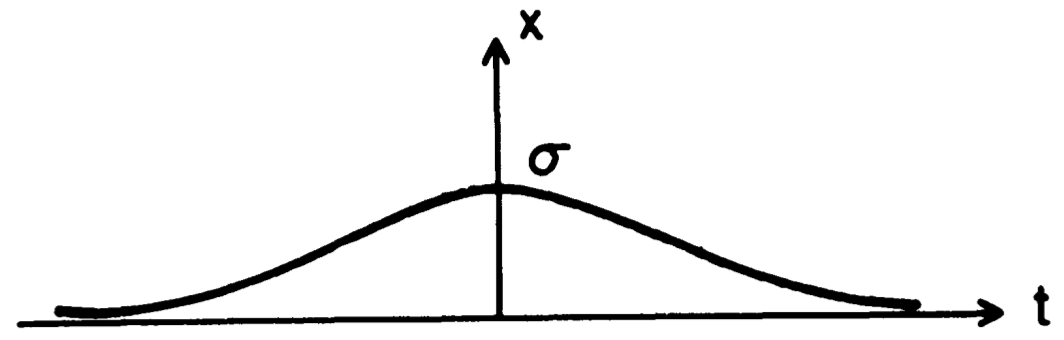
\includegraphics[width=0.5\textwidth]{instantonfig8.png}
    \caption{ \label{instantonfig8}}
  \end{figure}

\noindent {\kaishu{萨尔维阿蒂}}: 唉, 沙格列陀, 我恐怕你在三个地方出错了. 首先, 你所计算的项要远小于$\hbar^{2}$阶的项, 而你在计算过程中忽略了这样的项, 因此你没有理由保留它. 其次, 通过你的概述, 我看到这个回弹有个极大值; 而本征函数$x_{1}$正比于回弹的时间导数, 所以有一个节点. 因此它不是本征值最低的本征函数, 并且必然有一个本征值很低的无节点本征函数$x_{0}$, 这就是说, 必然有一个负本征值. $K$反比与本征值平方根之积, 因此是纯虚的. 最后, 你所研究的态由于势垒隧穿而变得不稳定, 因此你尝试计算的本征值不在哈密顿量的频谱中.

\noindent {\kaishu{沙格列陀}}: 你所说的都是正确的, 但我觉得你的批评也恰好指出了如何修正这个计算. 非稳态的能量有一个虚部; 因此只能期待$K$应该是纯虚的. 更进一步, 尽管我所计算的项相比于$E_{0}$的实部是可忽视的项, 但它是$E_{0}$虚部的领头贡献. 因此, 方程\eqref{instanton2.48}的修正版是
\begin{equation}
    \operatorname{Im}E_{0}= \Gamma/2= \hbar \lvert K \rvert \me^{-S_{0}/\hbar} \:, \label{instanton2.49}
\end{equation}
其中, 和通常一样, $\Gamma$是非稳态的展宽.

正如你所看到的, 这两个托斯卡纳人像往常一样机智敏捷, 然而他们的论证(也像往常一样)有点马虎. 沙格列陀丢了一个因子$\tfrac{1}{2}$; 正确的答案是
\begin{equation}
    \Gamma= \hbar \lvert K \rvert \me^{-S_{0}/\hbar} \:. \label{instanton2.50}
\end{equation}
为了证明它需要一个比沙格列陀更仔细的论证. 关键点是萨尔维阿蒂的观察: 非稳态的能量不是$H$的本征值; 事实上, 只能通过解析延拓来定义它. 
接下来我们来做这样的延拓.

为了让论述尽可能简单, 我们不考虑对全部函数空间的积分, 而只是对函数空间中的某个路径积分, 用实变量$z$参数化这个路径, 就有
\begin{equation}
    J=\int \dif z\: (2\pi\hbar)^{-1/2}\me^{-S(z)/\hbar} \:, \label{instanton2.51}
\end{equation}
其中$S(z)$是沿着这个路径的作用量. 特别地, 我们选择图\ref{instantonfig9}所示的路径. 这个路径包含两个出现在实际问题中的重要函数: 在$z=0$处的函数$x(t)=0$以及在$z=1$处的回弹. 更进一步, 这个路径在$z=1$处的切矢量是$x_{0}$. 因此这个路径从``最危险''的方向经过回弹这个函数, 即与负本征值相联系的方向, 而$z=1$是$S$的极大值, 如图\ref{instantonfig10}所示. 


  \begin{figure}[h]
    \centering
    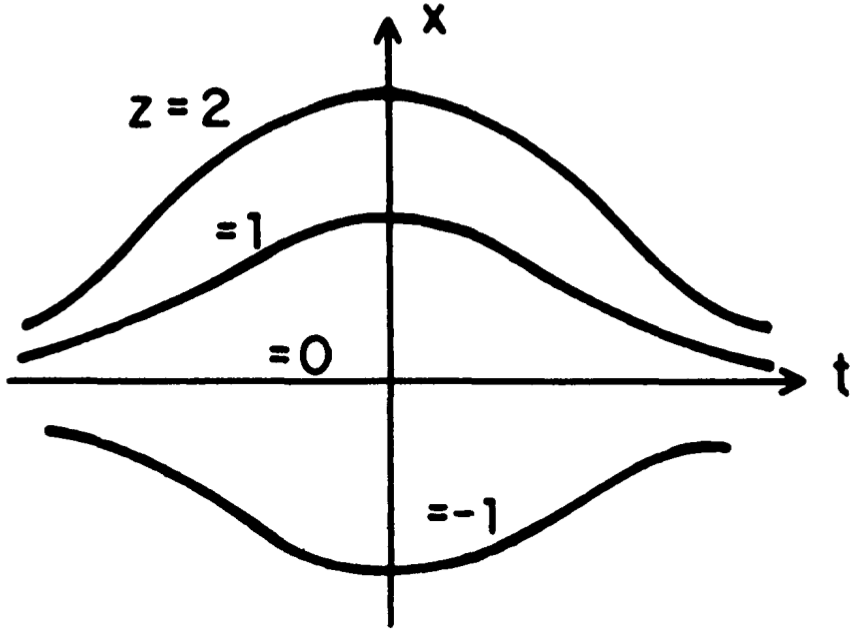
\includegraphics[width=0.5\textwidth]{instantonfig9.png}
    \caption{ \label{instantonfig9}}
  \end{figure}
\begin{tcolorbox}
    \begin{remark}
        这里稍微做一些解释. 我们把这个路径上的函数记为$x(z,t)$. 上面的条件相等于说$x(0,t)=0$以及$x(1,t)$是回弹解. 更进一步, 我们在$x(1,t)$附近展开作用量$S$:
        \[
        S(x(z,t))= S(x(1,t))+(x(z,t)-x(1,t))  \cdot \frac{\delta^{2}S}{\delta x^{2}}\biggr\vert_{x=x(1,t)}\cdot (x(z,t)-x(1,t))  
        \]
        这里的一阶导数由于经典运动方程为零, 而$(x(z,t)-x(1,t))=(z-1)\partial_{z}x(1,t)$, 我们把$\partial_{z}x(1,t)$展到$\delta^{2}S/\delta x^{2}$的本征函数, 这些本征函数只有$x_{0}$的本征值为负, 在这个方向上,
        \[
            S(x(z,t))=   S(x(1,t))-c_{0}\bigl((z-1)x_{0}\bigr)^{2}.
        \]
        因为$c_{0}$为正, 所以$S$迅速减小, 那么$\exp(-S/\hbar)$会指数增长, 因此称其为最危险的方向.
    \end{remark}    
\end{tcolorbox}
\noindent 随着$z$趋于无穷, 由于函数在转折点之后($V<0\,$)区域停留的时间越来越长, $S$趋于负无穷大; 这暗示了方程\eqref{instanton2.51}发散的很厉害.

\begin{figure}[h]
    \centering
    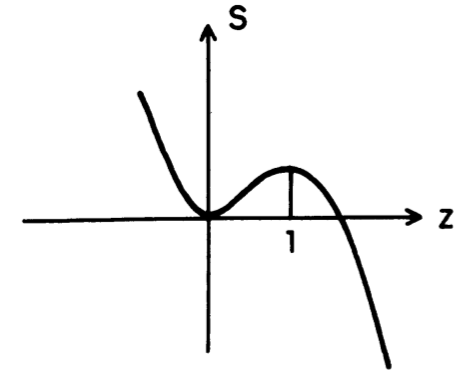
\includegraphics[width=0.5\textwidth]{instantonfig10.png}
    \caption{ \label{instantonfig10}}
  \end{figure}

如果$x=0$是$V$的绝对最小值, 这就是说, 如果$V$如图\ref{instantonfig11}(a)所示, 对于函数空间的同一路径, 情况将如图\ref{instantonfig11}(b)所示, 也就不会有方程\eqref{instanton2.48}中的发散. 现在我们解析地改变$V$使得我们从这个情况回到感兴趣的情况. 为了保持积分收敛, 我们必须把积分围道的右半端扭到复平面中. 如何改变积分围道依赖于如何将一个势变到另一个势的解析细节. 在图\ref{instantonfig12}中, 我们假定积分围道被扭到了上半平面. 使用最速下降法的标准处理, 将围道选取成: 沿着实轴从负无穷到鞍点$z=1$, 然后跑到复平面. 这个积分也就获得了虚部; 在最速下降的近似中
\begin{align}
    \operatorname{Im} J &= \operatorname{Im} \int_{1}^{1+\mi\infty} \dif z\: (2\pi\hbar)^{-1/2} \exp\Bigl(-S(1)/\hbar- \tfrac{1}{2}S''(1)(z-1)^{2}/\hbar\Bigr) \nonumber \\
    &=\tfrac{1}{2}\me^{-S(1)/\hbar} \bigl\lvert S''(1)\bigr\rvert^{-1/2} \:. \label{instanton2.52}
\end{align}
注意这个$\tfrac{1}{2}$因子; 它出现是因为积分围道只取了高斯峰的一半. (如果把积分围道扭到下半平面, 那么这个虚部就会有一个额外的符号).

\begin{figure}[h]
    \centering
    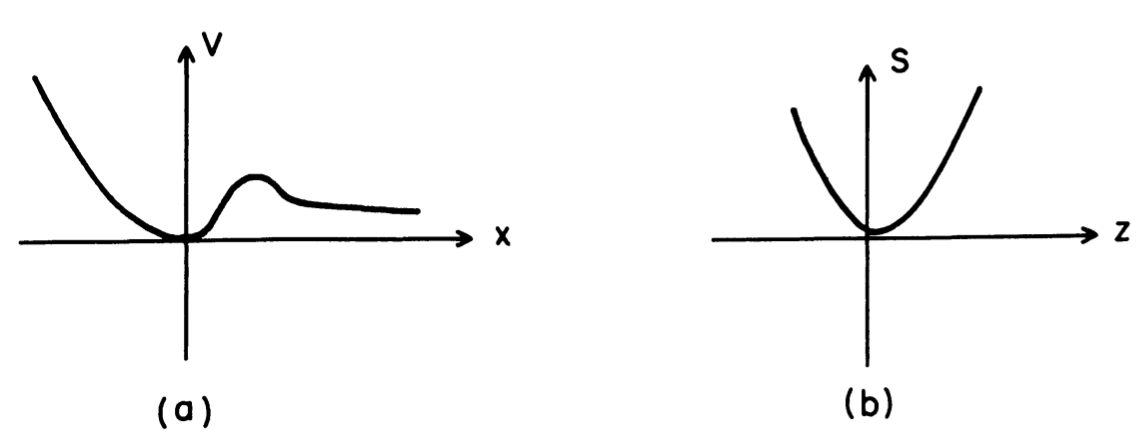
\includegraphics[width=0.9\textwidth]{instantonfig11.png}
    \caption{ \label{instantonfig11}}
  \end{figure}

  \begin{figure}[h]
    \centering
    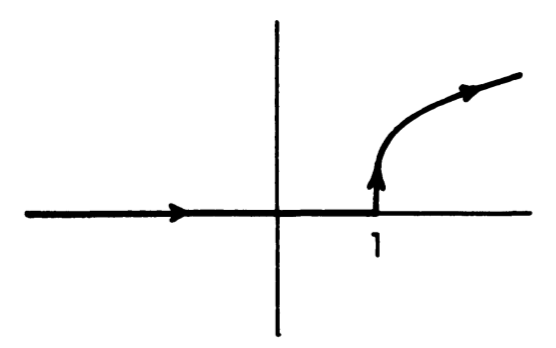
\includegraphics[width=0.5\textwidth]{instantonfig12.png}
    \caption{ \label{instantonfig12}}
  \end{figure}

我们到现在为止所研究的都是一维积分, 但由于与路径垂直的方向所联系的本征值都是非负的, 所以它们的泛函积分是平庸的. 以这种方式我们就获得了沙格列托的结果\eqref{instanton2.49}, 不同之处是对于负本征值有一个额外的$\tfrac{1}{2}$因子.


\section{规范场论中的真空结构}

\subsection{冷饭} \label{instanton:sec3.1}

这个小节主要回顾规范场论的一些基本知识, 并确定一些符号约定.

\paragraph*{李代数} 李代数的表示是$N$个反厄密矩阵$T^{a}$, $a=1,\ldots,N$, 的集合, 他们满足方程
\begin{equation}
    [T^{a},T^{b}]= c^{abc} T^{c} \:, \label{instanton3.1}
\end{equation}
其中$c$是某个紧李群$G$的结构常数. 总可以选择$T$使得$\operatorname{Tr}(T^{a}T^{b})$正比于$\delta^{ab}$, 而比例常数可能正比于表示. 嘉当内积定义成
\begin{equation}
    (T^{a},T^{b}) = \delta^{ab} \:. \label{instanton3.2}
\end{equation}
因此它正比于矩阵乘积的迹.

接下来来确定结构常数和$T$. 对于主要要处理的$SU(2)$, 选择$c^{abc}$为$\varepsilon^{abc}$. 因此, 对于同位旋表示,
\begin{equation}
    T^{a} = -\mi\sigma^{a}/2 \:, \label{instanton3.3}
\end{equation}
其中$\sigma$是泡利矩阵. 在这个情况下,
\begin{equation}
    (T^{a},T^{b})=-2\operatorname{Tr}(T^{a}T^{b}) \:. \label{instanton3.4}
\end{equation}

我们偶尔会讨论$SU(n)$, 特别是$SU(3)$. 对于它们, 结构常数和$T$的选择会使得它们对$SU(2)$子群与上面的选择相同. 因此, 对于$SU(3)$, $T^{a}$是$-\mi\lambda^{a}/2$, 其中$\lambda$是盖尔曼矩阵.

\paragraph*{规范场} 规范势是一组矢量场$A_{\mu}^{a}(x)$. 接下来定义矩阵值矢量场$A_{\mu}(x)$,
\begin{equation}
    A_{\mu}=gA_{\mu}^{a}T^{a} \:, \label{instanton3.5}
\end{equation}   
其中$g$是规范耦合常数. 场强张量$F_{\mu\nu}(x)$定义成
\begin{equation}
    F_{\mu\nu} = \partial_{\mu}A_{\nu}- \partial_{\nu}A_{\mu} + [A_{\mu},A_{\nu}] \:. \label{instanton3.6}
\end{equation}
纯规范场理论的欧几里得作用量是
\begin{equation}
    S= \frac{1}{4g^{2}} \int \dif^{4}x\: (F_{\mu\nu},F_{\mu\nu}) \:. \label{instanton3.7}
\end{equation}
有时简写成
\begin{equation}
    S=\frac{1}{4g^{2}} \int (F^{2}) \:. \label{instanton3.8}
\end{equation}

\paragraph*{规范变换} 规范变换是一个从欧几里得空间到规范群$G$的函数$g(x)$. 写成方程就是
\begin{equation}
    g(x) = \exp \bigl( \lambda^{a}(x)T^{a}\bigr) \:, \label{instanton3.9}
\end{equation}
其中$\lambda$是任意函数. (这里不要与耦合常数$g$相混淆.) 在这样一个变换下
\begin{equation}
    A_{\mu} \to g A_{\mu} g^{-1} +g \partial_{\mu} g^{-1} \:, \label{instanton3.10}
\end{equation}
以及
\begin{equation}
    F_{\mu\nu} \to g F_{\mu\nu} g^{-1} \:. \label{instanton3.11}
\end{equation}
因此$S$是规范不变的. 如果$F_{\mu\nu}$为零, 那么$A_{\mu}$是0的规范变换; 这就是说
\begin{equation}
    A_{\mu} = g\partial_{\mu}g^{-1} \:. \label{instanton3.12}
\end{equation}

\paragraph*{协变导数} 场强张量的协变导数定义成
\begin{equation}
    D_{\lambda}F_{\mu\nu} = \partial_{\lambda}F_{\mu\nu} + [A_{\lambda}, F_{\mu\nu}] \:. \label{instanton3.13}
\end{equation}
作用量\eqref{instanton3.7}给出运动方程
\begin{equation}
    D_{\mu} F_{\mu\nu} =0 \:. \label{instanton3.14}
\end{equation}
对于给定的场$\psi$, 假定它服从规范变换
\begin{equation}
    \psi \to g(x) \psi \:, \label{instanton3.15}
\end{equation}
那么$\psi$的协变导数
\begin{equation}
    D_{\mu}\psi = \partial_{\mu} \psi +A_{\mu} \psi
\end{equation}
以相同方式进行变换.

\subsection{缠绕数}

我们为什么研究作用量是有限值的规范场构型? 想当然的答案是, 作用量无限大的场构型有$\me^{-S/\hbar}=0$, 所以它们对泛函积分是不重要的. {\kaishu{这是错的}}. 实际上有限作用量的构型不重要; 更确切一些, 它们是函数空间的零测集. 我们对作用量有限的场构型感兴趣的唯一原因是我们想做半经典近似, 而如果我们把作用量无限大的场构型选做高斯积分的中心点, 那么它确实会给出零.
\begin{tcolorbox}
  \begin{remark}
    这里用有限维空间中的鞍点近似法来做一些解释说明:
    \begin{equation*}
        \int_{\mathbb{R}^{n}} g(x)\me^{\mi k f(x)} \dif x \simeq \sum_{x_{0}\in \Sigma} \me^{\mi k f(x_{0})}
        \bigl| \det (\operatorname{Hess}(f))\bigr|^{-1/2} \me^{\pi\mi \operatorname{sgn}(\operatorname{Hess}(f))/4}
        \biggl(\frac{2\pi}{k}\biggr)^{n/2}g(x_{0})
    \end{equation*}
这里的$\operatorname{Hess}(f)$是指$\partial^{2} f/\partial x_{i}\partial x_{j}$构成的海赛矩阵, 而$\operatorname{sgn}(\operatorname{Hess}(f))$是海赛矩阵的正本征值个数与负本征值个数之差, $\Sigma$则是临界点的个数.

上面所说的``有限作用量的构型是函数空间的零测集''就等同于这里的$\Sigma$是$\mathbb{R}_{n}$的零测集, 诚然在上式右边去掉这些临界点并不会对积分有影响, 但这里实际上关心的是积分关于临界点的展开, 而这样的展开仅在$k\to \infty$时才是有效的.
  \end{remark}  
\end{tcolorbox}

作用量积分的收敛性是由$A_{\mu}$在$r$很大时的行为决定的, 其中$r$是欧几里得空间中的径向变量. 为了使讨论尽可能简单, 假定$r$很大时, $A_{\mu}$可以展成$r$的负幂次的渐进级数. 因此为了使作用量有限, $F_{\mu\nu}$在$r$很大时必须比$1/r^{2}$衰减得要快; 这就是说, $F_{\mu\nu}$必须是$O(1/r^{3})$. 这暗示了$A_{\mu}$是$O(1/r^{2})$, 但这还不完全: $F_{\mu\nu}$为零只能给出$A_{\mu}$是零的规范变换. 因此$A_{\mu}$形如
\begin{equation}
    A_{\mu} = g \partial_{\mu} g^{-1} + O(1/r^{2}) \:, \label{instanton3.17}
\end{equation}
其中$g$是从4维空间到群$G$的$O(1)$函数, 这就是说, 它是角变量的函数.

\begin{remark}
这里的$g(x)$是紧群$G$上的元素, 所以它最多是$O(1)$的, 我们这里只关心$A_{\mu}$在$r\to\infty$时行为, 所以$g$只需要是角变量的函数.    
\end{remark}

因此, 每个作用量有限的场构型都会联系到角变量的一个群元值函数, 也就是说, 一个三维超球面$S^{3}$到规范群$G$的映射. 当然, 这个分配不是规范不变的. 在规范变换$h(x)$下,
\begin{equation}
    A_{\mu } \to h A_{\mu}h^{-1} + h \partial_{\mu}h^{-1} \:. \label{instanton3.18}
\end{equation}
因此,
\begin{equation}
    g\to hg + O(1/r^{2}) \:. \label{instanton3.19}
\end{equation}
\begin{tcolorbox}
    把方程\eqref{instanton3.17}代入\eqref{instanton3.18}右边, 得到
    \begin{align*}
        A_{\mu} &\to hg(\partial_{\mu}g^{-1})h^{-1} +h\partial_{\mu}h^{-1} \\
        &= hg \Bigl( (\partial_{\mu}g^{-1})h^{-1} +g^{-1}\partial_{\mu}h^{-1}\Bigr) =hg \partial_{\mu} (g^{-1}h^{-1}) \:. 
    \end{align*}
    即方程\eqref{instanton3.19}
\end{tcolorbox}

如果我们能选择$h$使得它在无穷远处等于$g^{-1}$, 我们可以把$g$变换到1然后从方程\eqref{instanton3.17}中消掉它. 然而, 这一般是不可能的. 
原因是$h$不仅要是无穷远处的超球面上的连续函数, 也得在整个四维空间连续, 也就是说, 沿着$r$把整个四维空间划成逐层嵌套的超球面, 在这些连续变换的超球面上, $h$是连续的. 特别地, $h$在原点必须是一个常数. 因此, 无穷远处的$h$不可能是$S^{3}$上的一般函数, 而是可以通过连续形变可以从常函数得到的连续函数. 由于任何常数规范变换都可以从恒等变换做连续形变得到(所有规范群都是连通的), 我们也可以说无穷远处的$h$可以通过对$h=1$做连续形变得到.

给定从一个拓扑空间到另一个拓扑空间的两个映射, 如果一个映射可以连续形变到另一个, 数学家称这两个函数是“同伦的”或者“处在同一个同伦类中”. 我们刚才证明了我们可以通过规范变换把$g(x)$变换到任何与$g(x)$同伦的映射, 但我们无法把它变换到另一个同伦类中的函数. 因此, 与有限作用量场构型相联系的不是$S^{3}$到$G$的映射, 而是这种映射的同伦类. 我们的任务是对物理上感兴趣的$G$找到这些同伦类.

我们先来做个热身练习, 考虑一个几何可视化的简化版. 我们将处理最简单的规范群, $U(1)$. 这样规范场论就是普通的电磁理论. (然而, 我们这里所采用的符号约定是\ref{instanton:sec3.1}节中确定的那些, 因此$A_{\mu}$将是纯虚的.) 另外, 我们将考虑二维空间而不是四维空间. 我们仍然要研究满足方程\eqref{instanton3.17}的场, 尽管这个条件不再是作用量有限的结果. 由于我们处理的是二维空间, 所以取代前面的超球面$S^{3}$, 我们这里面对的是一个圆$S^{1}$.

现在开始处理:
\begin{enumerate}
    \item $G$是复平面中的单位圆; 因此, 从拓扑上将, $G$也是$S^{1}$, 所以我们必须研究从$S^{1}$到$S^{1}$的映射的同伦类. 我们将按照传统方式用在$0$到$2\pi$之间取值的$\theta$来标记空间中的圆, 即映射的定义域.
    \item 定义一些从$S^{1}$到$S^{1}$的标准映射. 一个是平庸映射,
    \begin{subequations} \label{instanton3.20}
        \begin{gather}
            g^{(0)}(\theta)=1 \:. \label{instanton3.20a} \\
        \intertext{另一个是单位映射,}
            g^{(1)}(\theta) = \me^{\mi\theta} \:. \label{instanton3.20b}\\
        \intertext{它们都是如下映射族}
            g^{(\nu)}(\theta) = [g^{(1)}(\theta)]^{\nu} = \me^{\mi\nu\theta}  \tag{3.20c} \label{instanton3.20c} 
        \end{gather}  
    \end{subequations}
    的成员, 其中$\nu$是整数. $\nu$被称为``缠绕数''.
    \item 每个从$S^{1}$到$S^{1}$的映射同伦于映射\eqref{instanton3.20c}中的一个. 这是著名的事实$\pi_{1}(S^{1})=\mathbb{Z}$. 即圆的第一同伦群是整数加法群.
    \item 上述缠绕数可以有如下积分公式给出:
    \begin{equation}
        \nu = \frac{\mi}{2\pi} \int_{0}^{2\pi} \dif\theta\: g\frac{\dif }{\dif\theta} g^{-1}\:. \label{instanton3.21}
    \end{equation}
    对于标准映射\eqref{instanton3.20c}, 这显然是成立的. 这个量在连续变换下也是不变的. 这点可以通过考虑无限小形变来证明. 一个无限小的形变可以写成
    \begin{equation}
        \delta g =\mi (\delta\lambda) g\:, \label{instanton3.22}
    \end{equation}
    其中$\delta\lambda$是圆上的无限小实函数. 因此
    \begin{align}
        \delta\biggl(g\frac{\dif}{\dif\theta} g^{-1}\biggr) &= (\delta g)\frac{\dif}{\dif\theta} g^{-1}+
        g\frac{\dif}{\dif\theta} (\delta g^{-1})=\mi\delta \lambda \,g \frac{\dif}{\dif\theta} g^{-1} 
        -\mi g \frac{\dif}{\dif\theta} (\delta\lambda\,g^{-1}) \nonumber \\
        &=-\mi \frac{\dif}{\dif\theta} \delta\lambda \label{instanton3.23}
    \end{align}
    这里使用了$\delta g^{-1}= -g^{-1}(\delta g) g^{-1}$, 由此看出这不会对$\nu$产生影响.
    \item 如果
    \begin{subequations}
        \begin{gather}
        g(\theta) = g_{1}(\theta)g_{2}(\theta) \:, \tag{3.24a} \label{instanton3.24a} \\
    \intertext{那么}
        \nu= \nu_{1}+\nu_{2} \:. \tag{3.24b} \label{instanton3.24b}
        \end{gather}
    \end{subequations}
    证明是简单的: 对$g_{1}$做形变使得它在上半圆为1, 对$g_{2}$做形变使得它在下半圆为1.
    \item 我们定义
    \begin{equation}
        G_{\mu} =\frac{\mi}{2\pi} \varepsilon_{\mu\nu} A_{\nu} \:. \label{instanton3.25}
    \end{equation}
    通过方程\eqref{instanton3.17}和\eqref{instanton3.21},
    \begin{equation}
        \nu = \lim_{r\to\infty} \int_{0}^{2\pi} r \dif \theta\: \hat{r}_{\mu}G_{\mu} \:, \label{instanton3.26}
    \end{equation}
    其中$\hat{r}_{\mu}$是径向单位矢量. 因此通过高斯定理,
    \begin{equation}
        \nu = \int\dif^{2}x\: \partial_{\mu}G_{\mu} \:. \label{instanton3.27}
    \end{equation}
    这样,
    \begin{equation}
        \nu = \frac{\mi}{4\pi}\int\dif^{2}x\: \varepsilon_{\mu\nu}F_{\mu\nu} \:. \label{instanton3.27}
    \end{equation}
    \begin{remark}
        这里使用了$\hat{r}_{\mu}\varepsilon_{\mu\nu}A_{\nu}=\cos\theta A_{y}-\sin\theta A_{x}= r^{-1} g\partial_{\theta} g^{-1}$
    \end{remark}
\end{enumerate}

\subsection{多个真空}

\subsection{瞬子: 一般情形}

\subsection{瞬子: 特殊情形}

\section{$1+1$维中的阿贝尔Higgs模型}



\section{$U(1)$问题的't Hooft解决方案}

\subsection{介子失踪之谜}

\subsection{准备工作: 欧几里得费米场}

\subsection{准备工作: 手征沃德恒等式}

\subsection{QCD(幼儿版)}


\subsection{QCD(真实版)}

\subsection{杂录}


\section{假时空的命运}

\subsection{不稳定真空}

\subsection{回弹}

\subsection{薄壁近似}

\subsection{假真空的命运}

\subsection{行列式与重整化}

\subsection{待解答的问题}


\end{document}
